%
%	Plan de Gestión de Configuración del Software (GCS)
%

\documentclass[11pt, a4paper, twoside, titlepage]{article}
\usepackage[utf8x]{inputenc}
\usepackage[T1]{fontenc}
\usepackage[spanish]{babel}
\usepackage{lmodern}
\usepackage{anysize}
\usepackage[none]{hyphenat}
\usepackage[colorlinks, linkcolor=red]{hyperref}
\usepackage{glossaries}
\usepackage{glossaries-babel}
%\usepackage{lscape}
\usepackage[doc=gcs]{isdiedral}
%\usepackage{multicol}
%\usepackage{amsmath}
%\usepackage{float}

% Nombre del documento (para futuras referencias)
\newcommand*{\doctitle}{Plan de gestión de configuración del software}


%%% Configuraciones %%%
\marginsize{2.5cm}{2cm}{2cm}{2cm}

% Usa como familia tipográfica por defecto "Sans"
\renewcommand{\familydefault}{\sfdefault}

% Establece la profundidad hasta la cual se numeran los elementos de sección
\setcounter{secnumdepth}{4}

% Establece la profundidad de niveles de sección que aparece en el TOC
\setcounter{tocdepth}{4}

% Fija que la entrada del glosario se comporte como una subsección
\setglossarysection{subsection}

% Configuración de los encabezados
\encabezadodiedral{\doctitle}
\pagestyle{fancy}

\renewcommand*{\thepage}{\sffamily \roman{page}}


% Modelo copiado de los apuntes del tema 8 (páginas 93 a 95) IEEE Std. 730-2002

\title{\doctitle\\\textsl{Airline Common Environment}}
\author{Grupo Diedral}

% Metadatos del pdf
\hypersetup{
pdfinfo={
	Author={Grupo Diedral},
	Title={\doctitle},
	Subject={Airline Common Environment},
	Keywords={SQA;Airline Common Environment;Ingeniería del Software}
}
}

% Inclusión del glosario (gracias a David Peñas)
%
%	Plan GCS: Glosario
%

\PrerenderUnicode{ñ}
\PrerenderUnicode{ó}
\PrerenderUnicode{í}


\makeglossaries

\begin{document}

	% Cita inicial
	\fijacitainicial{Nada es permanente a excepción del cambio}{Heráclito de Éfeso, $\sim$ 500 a.C.}

	% Portada
	\portadaace{\doctitle}{2.0}

	\tableofcontents
	\newpage

	\iniciarnumeraciondiedral
	
	\section{Introducción} % Natalia
		\subsection{Propósito}
			El propósito del Plan de \gls{config_software} es establecer y mantener la integridad de los productos a desarrollar a través del proceso de software asociado. 
		\subsection{Alcance}
		\begin{itemize}
			\item Se \textit{identificarán y definirán los elementos del sistema}, controlando el posible cambio de estos durante todo su ciclo de vida, y se verificarán que sean correctos y completos.
			\item Se establecerá un protocolo de \textit{gestión de cambios} de estos elementos.
			\item Será la base de partida para que se pueda generar una buena \textit{calidad de software}.
			\item Ayudará a la comunicación y organización en el grupo de desarrollo o con personas ajenas al proyecto.
		\end{itemize}
			
		%\subsection{Definición de términos clave} Esto es el Glosario
		\subsection{Referencia}
			\nocite{IEEE828-1998}
			\nocite{PSMAN}
			Ver sección de {\itshape Referencias} al final del documento.
		
	\section{Gestión de la GCS} % Sandra
		\subsection{Organización}
		\subsection{Responsabilidades GCS}
		\subsection{Políticas, directivas y procedimientos aplicables}
	\section{Actividades de la GCS}
		\subsection{Identificación de la configuración} % Natalia
			En la siguiente sección se va a realizar la Identificación, nombrado y adquisición de \gls{ECS}.

			\subsubsection{Casos de Uso}
				\begin{enumerate}
					\item {\itshape \bfseries Descripción.}
						\begin{itemize}
							\item \textit{Tipo de ECS:} Documento.
							\item \textit{Identificador proyecto:} CU.
							\item \textit{Información de la versión y/o cambio:} Es el documento que más correcciones ha necesitado. Aquí se han introducido dos nuevos casos de uso de los que los desarrolladores desconocían su necesidad, se han estructurado las tablas de descripción de Casos de Uso y se ha puesto en común el mismo uso de tiempos verbales y otras cosas que no colapsaban visualmente bien.
						\end{itemize}

					\item {\itshape \bfseries Lista de recursos.}
						La principal lista de recursos de este documento será la base de información que el Cliente nos quiera dar acerca de el producto a desarrollar, puesto que este es el documento en el que, siguiendo el modelo de UML, se basará todo nuestro proyecto Software. Este es el motivo por el que se ha hecho un gran esfuerzo en la gestión de configuración y de calidad de este documento.
				\end{enumerate}

			\subsubsection{Especificación de requisitos Software}
				\begin{enumerate}
					\item {\itshape \bfseries Descripción.}
						\begin{itemize}
							\item \textit{Tipo de ECS:} Documento.
							\item \textit{Identificador proyecto:} SRS.
							\item \textit{Información de la versión y/o cambio:} Se han cambiado principalmente errores derivados de modificaciones en el documento de Casos de Uso. Además, también se han corregido errores de redacción, pequeñas contradicciones entre algunas partes del proyecto y se ha mejorado el documento gracias a revisiones de terceras personas desde otro punto de vista diferente.
						\end{itemize}

					\item {\itshape \bfseries Lista de recursos.}
						Principalmente el documento de la Especificación de Requisitos Software tiene como entidades requeridas al documento de Casos de Uso y al Prototipo, es decir, depende directamente de ellos.
				\end{enumerate}

			\subsubsection{Prototipo Gestión Externa}
			\begin{enumerate}
				\item {\itshape \bfseries Descripción.}
						\begin{itemize}
							\item \textit{Tipo de ECS:} Programa.
							\item \textit{Identificador proyecto:} Prototipo Externa.
							\item \textit{Información de la versión y/o cambio:} No ha habido cambios desde la primera versión que se entregó este prototipo.
						\end{itemize}

					\item {\itshape \bfseries Lista de recursos.}
						La principal fuente de referencia del \textit{Prototipo de Gestión Externa} es el \textit{Documento de Requisitos Software} puesto que todo prototipo bien especificado y para que pueda tener un buen diseño deberá cumplir los requisitos especificados anteriormente en la documentación.
				\end{enumerate}

			\subsubsection{Prototipo Gestión Interna}
			\begin{enumerate}
				\item {\itshape \bfseries Descripción.}
						\begin{itemize}
							\item \textit{Tipo de ECS:} Programa.
							\item \textit{Identificador proyecto:} Prototipo Interna.
							\item \textit{Información de la versión y/o cambio:} Ligeras modificaciones a la hora de visualizar el prototipo y cambios en la estructura del código de éste. No se han realizado grandes cambios por la proximidad que tiene para ser desechado y reemplazado por la implementación final del producto Software.
						\end{itemize}

					\item {\itshape \bfseries Lista de recursos.}
						\textit{(Ver lista de recursos de Prototipo Gestión Externa)}
				\end{enumerate}

			\subsubsection{Plan de Proyecto}
			\begin{enumerate}
				\item {\itshape \bfseries Descripción.}
						\begin{itemize}
							\item \textit{Tipo de ECS:} Documento.
							\item \textit{Identificador proyecto:} Plan de Proyecto.
							\item \textit{Información de la versión y/o cambio:} Habrá que corregir bastantes errores en la parte de \textit{Estimación de Puntos de Función}, como aumentar la especificación de la obtención de algunos \gls{DET} y la falta del cálculo de los PF totales por extravío del archivo al realizar la entrega. En la parte de \textit{Gestión de Riesgos}, modificaremos el diseño de tal forma que sea mejor comprensible para el lector. Y por último, en la parte de \textit{Planificación temporal}, intentaremos generar unos mejores gráficos con el \textit{Microsoft Project} o en su defecto intentaremos arreglarlo tomando otras alternativas en las que la visualización de los documentos generados sea más buena.
						\end{itemize}

					\item {\itshape \bfseries Lista de recursos.}
						El Plan de Proyecto tiene como subrecursos internos el \textit{Plan de Gestión de Riesgo}, el P\textit{lan de Estimación} y el \textit{Documento de Planificación temporal}, puesto que dicho plan está formado principalmente por estos tres.
				\end{enumerate}

			\subsubsection{Plan de Gestión de Configuración}
			\begin{enumerate}
				\item {\itshape \bfseries Descripción.}
						\begin{itemize}
							\item \textit{Tipo de ECS:} Documento.
							\item \textit{Identificador proyecto:} GCS.
							\item \textit{Información de la versión y/o cambio:} En esta primera versión de este documento se describirán las gestiones de Revisiones Software llevadas a cabo durante el proceso de modificaciones después de la última entrega.
						\end{itemize}

					\item {\itshape \bfseries Lista de recursos.}
						Este documento está ligado al \textit{Plan de Calidad}, pues estos dos se encargan de cosas comunes como gestión y verificación de que se realiza la modificación y revisión de documentos del proyecto.
				\end{enumerate}

			\subsubsection{Plan de Gestión de Calidad}
			\begin{enumerate}
				\item {\itshape \bfseries Descripción.}
						\begin{itemize}
							\item \textit{Tipo de ECS:} Documento.
							\item \textit{Identificador proyecto:} PGC.
							\item \textit{Información de la versión y/o cambio:} Dado que es la primera versión de este documento, principalmente indicará los caminos llevados a cabo para la supervisión y modificaciones de los errores detectados en las Revisiones del Plan de GCS. Se irá actualizando conforme se vayan realizando entregas y se vayan revisando documentos.
						\end{itemize}

					\item {\itshape \bfseries Lista de recursos.}
						Este documento está ligado al \textit{Plan de Gestión de Configuración} de la misma manera que anteriormente se ha comentado.
				\end{enumerate}

			\subsubsection{Otros}
				Algunos ECS importantes que no se van han desarrollado aún y que por tanto no se van a detallar en este documento son: Diagramas de colaboración de análisis, el documento de diseño, el manual de usuario, el plan de pruebas del sistema, documentos de diseño de base de datos, especificaciones de prueba del sistema\ldots

		\subsection{Contabilidad de estado de configuración} % Sandra
	\section{Recursos de la GCS} %Natalia
		\textbf{Herramientas técnicas y Software.}
			La principal herramienta en la que se va a basar la \textit{Gestión de Configuración del Software} será en el Repositorio de Documentación elegido para desarrollar el entorno de trabajo de los desarrolladores. Pese a los problemas resueltos que sucedieron antes de la última entrega (baja del Repositorio RiouxSVN) y que fueron resueltos gracias al desarrollo del Plan de Contingencia del riesgo identificado como \textit{"`Repositorio Inoperativo"'}, en las últimas entregas no han surgido granes conflictos de documentos. Así, la organización del nuevo repositorio AssemblaSVN ha quedado de la siguiente manera: \\
			\begin{center}
				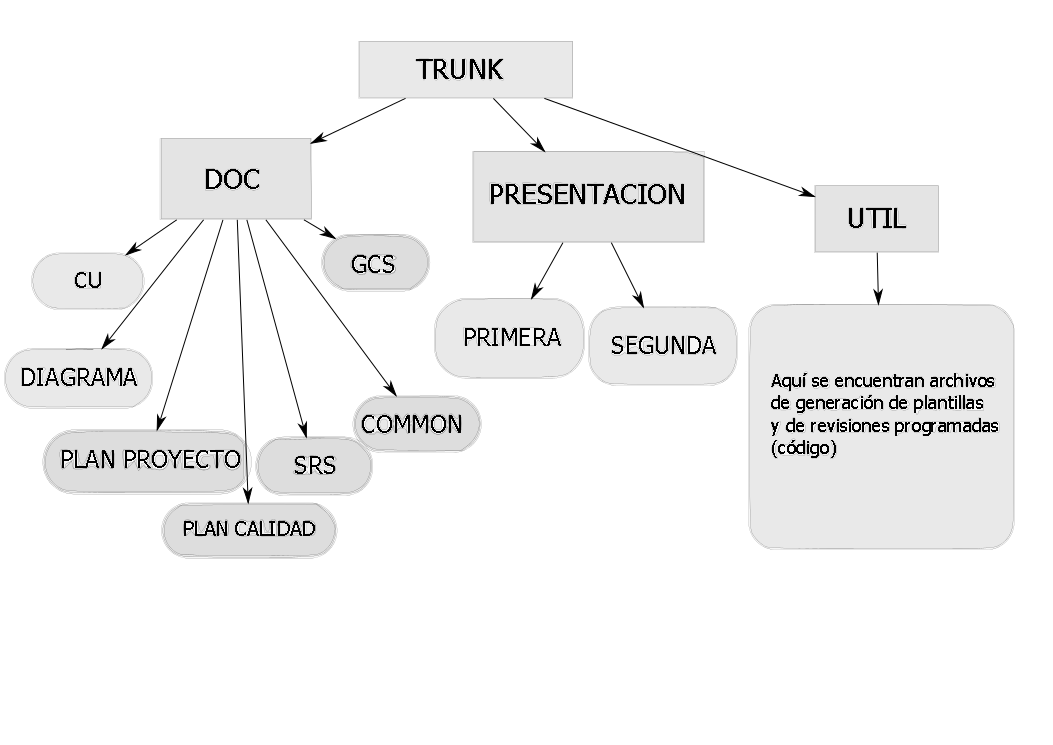
\includegraphics[scale=.4]{repositorio.png}
			\end{center}

	\section{Glosario}
		\printglossaries

	\newpage
	\bibliography{gcs}
	\bibliographystyle{plain}
\end{document}
